%assurances.tex

%\nisarcomm{trim, merge, move earlier...}

    %In Section~\ref{sec:introduction} we introduced the term \emph{assurances}. 
    An assurance is an AIA property or behavior that can either increase or decrease user trust. %of a human within a human-AIA trust relationship. 
    %As assurances are the main topic of this paper, and have received relatively little attention in trust literature, a more detailed definition and discussion is merited. 
    %\brettcomm{IS THERE ANYTHING IN PSYCHOLOGY RESEARCH??, mention \cite{Fogg1998-zf,Fogg2009-vb}} -- nra: there is a fundamental difference between persuasive computing and assurances as considered here -- persuasive computing deals with `nudging' users (whether consciously or subconsciously) to make certain decisions that are favored by designers. In some sense this requires manipulation of trust, but not necessarily calibration for user's own decision making. Might be worth mentioning later...but no need to mention this here...
    %
    The term `assurances' is perhaps earliest used in the context of human-AIA relationships by \citet{Sheridan1984-kx}. \citet{McKnight2001-fa} allude to this kind of feedback in e-commerce relationships as `Web Vendor Interventions' and mention some possible actions that might be used in this context, going so far as to these interventions to an online user's `Trusting Beliefs', `Trusting Intentions', and `Trust-Related Behaviors'. %(see Figure~\ref{fig:UserTrust}) 
    %of an online human user. 
    \citet{Corritore2003-gx} refer to assurances as `trust cues' that can influence how online users trust e-commerce vendors. \citet{Lee2004-pv} discuss `display characteristics', which are methods by which an autonomous systems can communicate information to an operator. More recently, \citet{Lillard2016-yg} provided a formal definition of assurances for autonomous systems that is similar to the one used here. %%; we have adapted their definition to be more general:    
%    \begin{description}
%        \item [Assurance:] An AIA property or behavior that either increases or decreases user trust.
%    \end{description}

%    \begin{figure}[htpb]
%        \centering
%        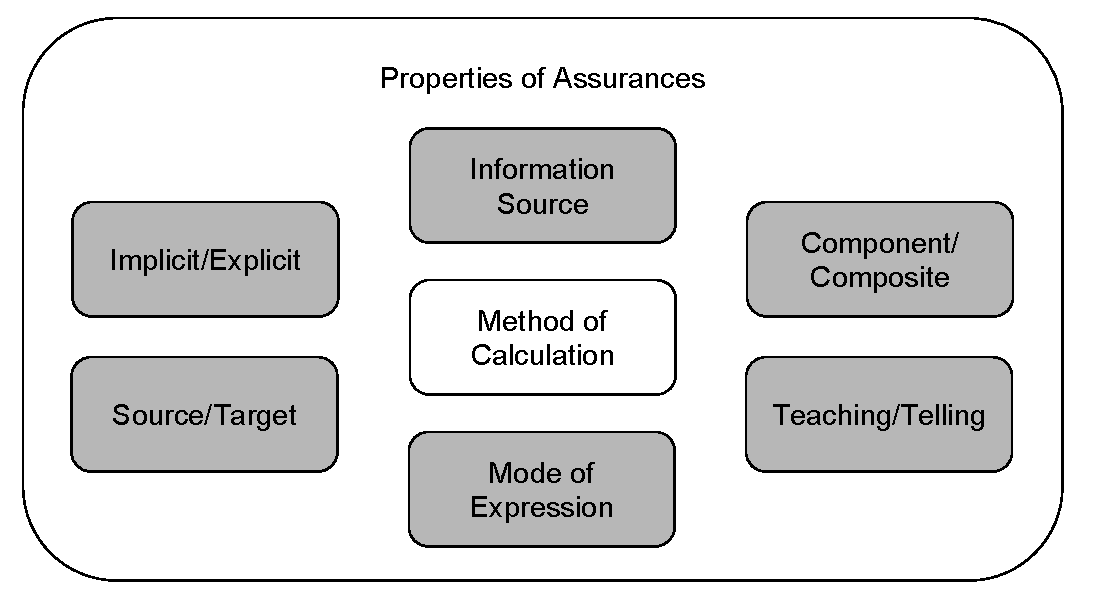
\includegraphics[width=0.6\linewidth]{Figures/Assurance_properties.pdf}
%        \caption{All assurances possess at least these properties (others likely exist as well).}
%        \label{fig:assurance_classification}
%    \end{figure}
%
%
    \begin{figure}[t]%[htpb]
        \centering
        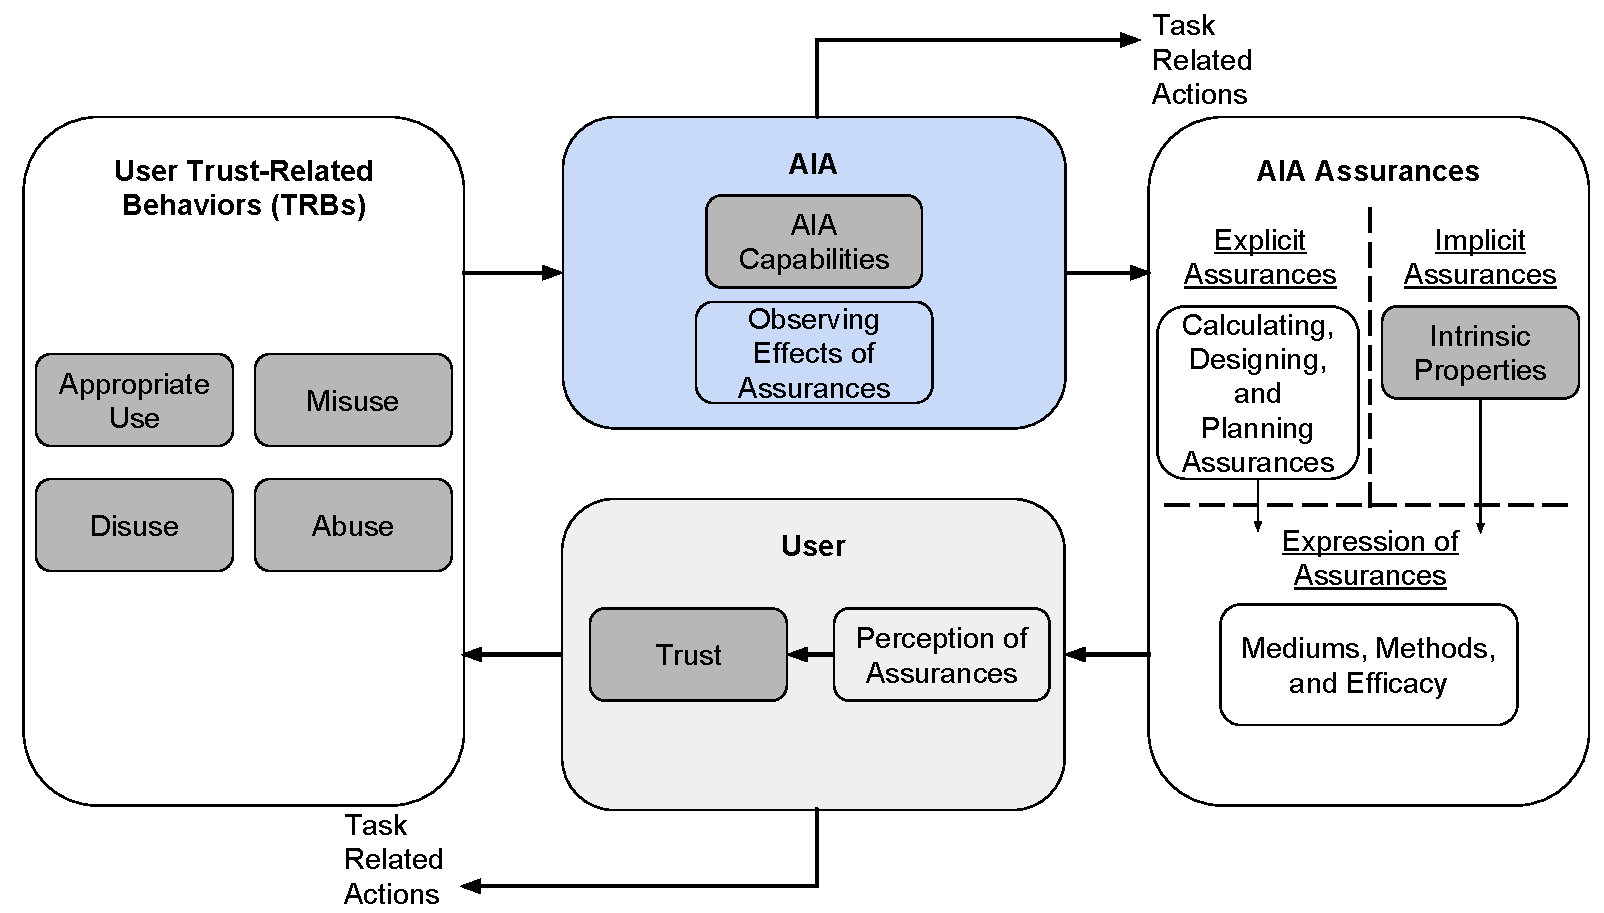
\includegraphics[width=0.6\linewidth]{Figures/RefinedTrust_one_way.pdf}
        \caption{Figure depicting the details of the human-AIA trust cycle.}
        \label{fig:refined_trust}
    \end{figure}

    \nisarcomm{for Brett todo: finish writing this section...}
    \brettcomm{Paragraph here that discusses Figure~\ref{fig:refined_trust}, how the boxes have been filled in by definitions that we have presented so far. Point out the details in the assurances box, and stuff like that} 
    
    %%\nisarcomm{other figure of assurances only is redundant given complete loop figure...complete loop figure is also a nice summary of the key definitions for the synthesis and thus a good setup to put survey into proper context -- a picture is worth a thousand words...}

    \brettcomm{Discuss the main taxonomy of the survey. Mention that other taxonomies are possible and are mentioned in the future work section\ldots Make clear that our survey is going pursue the taxonomy of algorithms that have been used to calculate assurances}

    %%\nisarcomm{I would leave this bit out (esp V&V part, since this is not correct to include) just end with last parag above}
    %%Researchers in the fields of AI, ML, data science, and robotics will recognize terms like \emph{interpretable}, \emph{comprehensible}, \emph{transparent}, \emph{verified and validated} (V\&V), \emph{certified}, and \emph{explainable AI}, with respect to the models or performance of a designed AIA. A key claim of this paper is that, \textbf{from a high level, all of these approaches have the same underlying aim: for a user to be able to trust an AIA to operate in a certain way, and (based on that trust) engage the AIA with an appropriate set of behaviors}. These fields have thus each developed mechanisms to assure or calculate assurances that are similar on a fundamental level. 
